\subsection{Алгоритм для смешанного языка Дика}

% Смешанный язык Дика
\begin{definition}
    \TODO: нормально определение в секции с определениями

    Пусть у нас есть два языка Дика $D_i$ и $D_j$ над разными алфавитами (например, в одном~--- $(_i, )_i$, а в другом $[_i, ]_i$). Тогда в смешанном языке Дика $D_i \bigodot D_j$ лежат слова, такие что, если рассмотреть проекции на алфавиты $D_i$ и $D_j$, то это корректные слова из $D_i$ и $D_j$ (\textit{Ужасно..})

    Пример: ``$([(])[[(]))]$''~--- корректное слово из $D_1 \bigodot D_1$. 
\end{definition}

\begin{note}
    $D_i \bigodot D_j$~--- это на самом деле пересечение двух КС языков (как обычные языки Дика, но там где $\eps$, ещё можно скобки второго типа \TODO).

    Однако КС-языки не замкнуты относительно пересечения, более того, проверять непустоту пересечения двух КС-языков undecidable (\TODO: link)
\end{note}

\begin{lemma}~\cite{Li21}
    В двунаправленном графе, если между парой вершин $(u, v)$ существует какой-то $D_1 \bigodot D_1$ путь, то существует и такой путь, на котором в любой момент времени вложенность хотя бы одного типа скобок не превышает $6n$.

    \textit{В доказательстве крутят циклы, в подробности я не вдавалась}
\end{lemma}

\begin{figure}[H]
    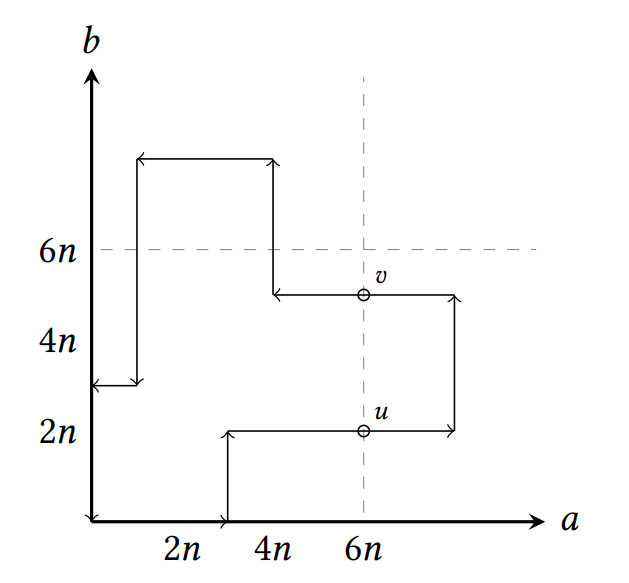
\includegraphics[width=0.75\linewidth]{img/6n_6n_path}
    \caption{Путь (кродеться)}
    % \label{img:dyck_rsm}
\end{figure}

\begin{note}
    То есть путь можно искать следующего вида: он в основном ходит внутри квадрата $[0, 6n] \times [0, 6n]$, иногда вылезая из него, но только по одной координате.

    Т.е. нужно разобрать отдельно две сущности: куски путей внутри квадрата, и куски путей, которые выходят погулять.
\end{note}

Вооружившись этим знанием, соорудим вот какой алгоритм:

\begin{enumerate}
    \item {\bf Часть про пути в квадратике}

    Помним (из прошлой главы), что если хотим решать $D_1$-достижимость, зная, что вложенность ограничена, можем это с помощью ДКА делать.

    \begin{figure}[H]
        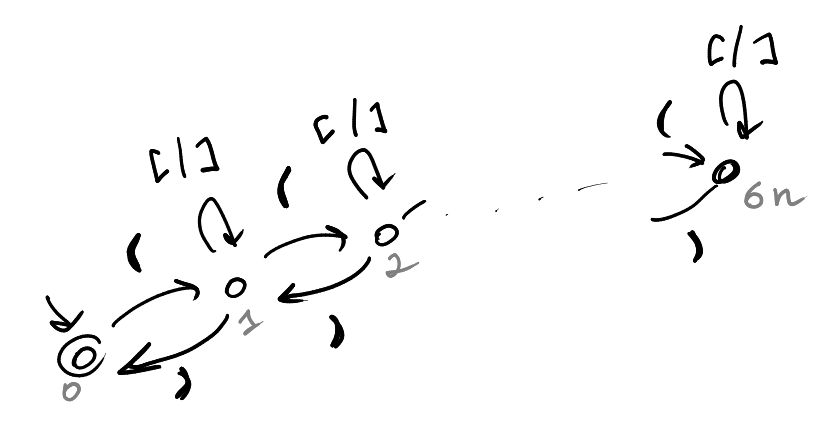
\includegraphics[width=0.75\linewidth]{img/dyck_1_1_dfa}
        \caption{ДКА для круглых скобок}
        % \label{img:dyck_rsm}
    \end{figure}

    Строим такие ДКА для обоих типов скобок. Т.к. и тот, и другой регулярный, то можем их прекрасно пересечь с нашим графом. 

    Получается такой граф троек $(u, b, p)$ (вершина, баланс квадратных скобок, баланс круглых скобок) на $\O(n^3)$ вершинах и $\O(n^2 m)$ рёбрах.

    Ещё в нём будут $\eps$-рёбра, найденные второй частью алгоритма. Эти рёбра имеют вид $(u, 6n, a) \to (v, 6n, b)$. Для всех возможных пар $a/b$ и $u/v$ их $\O(n^4)$.

    Т.к. входной граф двунаправленный, то полученное произведение будет неориентированным (\textit{это не совсем тривиально, но понятно}), значит достижимость на нём можно искать просто dfs'ом за $\O(n^4)$.

    \item {\bf Часть про гуляющие пути}

    В какой момент пути идут гулять? Когда вложенность одной из скобок ровно $6n$. А когда возвращаются? Тоже когда ровно $6n$. А во все моменты между $\ge 6n$. 

    То есть хотим искать такие пути, что по одной скобке они просто сбалансированы ($6n \path 6n$), а по другой какие попало, но всё время не больше $6n$ ($a \path b$, $a, b \le 6n$). 

    Опять-таки, решаем через пересечение языков. Первый~--- наш граф ($L_1$). Второй~--- просто язык Дика ($L_2$) (опять-таки с оговорками про то, что скобочка другого типа~--- это то же, что и $\eps$). Третий~--- пути Дика, начинающиеся в балансе $a$ и заканчивающиеся в балансе $b$ ($L_3$) (решаем для всех возможных пар балансов, чтобы рёбра провести). Давайте решать отдельно для каждого $a$, то есть нам нужен язык Диковых последовательностей со стартовым балансом $a$, таких, что их баланс не уходит в минус. Язык, опять-таки регулярный. 

    Дальше пересекаем. Сначала пересекаем $L_1 \cap L_2$. Это просто прямое произведение~--- граф пар $(u, b)$ (для каждого $a$ отдельно, снаружи всего это как бы фор по $a$). Вершин в нём $\O(n^2)$, рёбер $\O(n m)$. Теперь нужно это ещё пересечь с $L_3$. Ну так это же просто язык Дика, а Дикову достижимость мы за $\O(m^{*} \alpha)$ на двунаправленных графах решаем (а произведение $L_1 \cap L_2$ как раз двунаправленное). 

    Получаем $\O(n \cdot n m^{*} \alpha) = \O(n^4 \alpha)$.

\end{enumerate}

\subsection{Выводы и результаты по главе}